\documentclass{beamer}

\usepackage{amsmath}
\usepackage{amssymb}
\usepackage{mathtools}
\usepackage{amstext}
\usepackage{amsthm}
\usepackage{fancyhdr}
\usepackage{siunitx}
\usepackage{physics}

\usepackage{hyperref}


\usepackage{graphicx}
\usepackage{float}
\graphicspath{{figures/}} %Setting the graphicspath
\usepackage{float}
\usepackage{caption}
\usepackage{subcaption}

% To work with inkfigures
\usepackage{import}
\usepackage{pdfpages}
\usepackage{transparent}
\usepackage{xcolor}

\newcommand{\angstrom}{\textup{\AA}}
%\numberwithin{equation}{section}
\renewcommand\thesubsection{\alph{subsection})}
\renewcommand\thesubsubsection{\Roman{subsubsection}}
\newcommand{\s}{\hspace{0.1cm}}

%\usetheme{AnnArbor}
%\usetheme{Antibes}
%\usetheme{Bergen}
%\usetheme{Berkeley}
%\usetheme{Berlin}
%\usetheme{Boadilla}
%\usetheme{boxes}
%\usetheme{CambridgeUS}
%\usetheme{Copenhagen}
%\usetheme{Darmstadt}
%\usetheme{default}
%\usetheme{Frankfurt}
%\usetheme{Goettingen}
%\usetheme{Hannover}
%\usetheme{Ilmenau}
%\usetheme{JuanLesPins}
%\usetheme{Luebeck}
\usetheme{Madrid}
%\usetheme{Malmoe}
%\usetheme{Marburg}
%\usetheme{Montpellier}
%\usetheme{PaloAlto}
%\usetheme{Pittsburgh}
%\usetheme{Rochester}
%\usetheme{Singapore}
%\usetheme{Szeged}
%\usetheme{Warsaw}

\usefonttheme[onlymath]{serif}
% Astronomy
\DeclareSIUnit\parsec{pc}
\DeclareSIUnit\lightyear{ly}


\institute[] % (optional, but mostly needed)
{
		Département de Physique\\
		Université de Montréal
}
\title{Mesure de $H_0$}
\subtitle{Détermination du potentiel de Fermat de la lentille RXJ1131-1231}

\author{Alexandre Adam, \\ 
        Charles Wilson}

\date{PHY6669 -- Cosmologie}

\AtBeginSubsection[]
{
  \begin{frame}<beamer>{Résumé}
	\tableofcontents[currentsection,currentsubsection]
  \end{frame}
}

\usepackage[authoryear]{natbib}
\bibliographystyle{abbrvnat}
%\bibliographystyle{apacite}
\captionsetup{labelformat=empty,labelsep=none}

\begin{document}

\begin{frame}
	\titlepage
\end{frame}


\begin{frame}{Résumé}
	\tableofcontents
\end{frame}

\section{Contexte}
\subsection{Mesures}

\begin{frame}{Mesures}{Planck (2018) + $\Lambda$CDM}
        \begin{figure}[H]
                \centering
                \includegraphics[width=\textwidth]{TT_power_spectra_Planck2018}
                \caption{Mesure indirecte: $\boxed{100h = 67.36 
                        \pm 0.54\,\, (0.8\%)}$ à $z \gtrsim 1100$
                \footnote{\citet{PlanckCollaboration2018}}}
        \end{figure}
        	
\end{frame}

\begin{frame}{Mesures}{Sh0es (Riess \textit{et al.})}
        \begin{figure}[H]
                \centering
                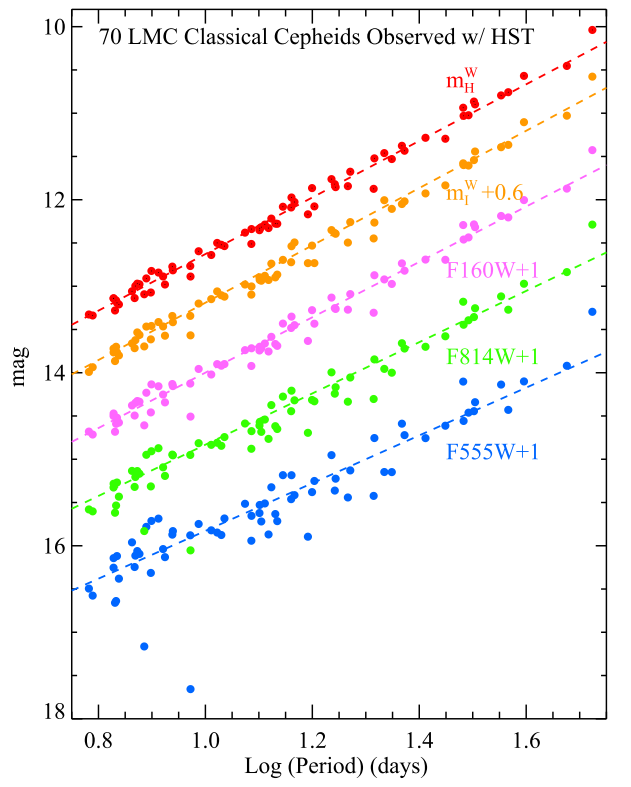
\includegraphics[width=0.4\textwidth]{Sh0es_mesure}
                \caption{Mesure directe: $\boxed{100h = 74.03 \pm 1.42\,\,(1.9\%)}$ à $z\ll 1$
                \footnote{\citet{Riess2019}}}
        \end{figure}
\end{frame}

\begin{frame}{Mesures}{H0LiCOW (Suyu \textit{et al.})}
        \begin{figure}[H]
                \centering
                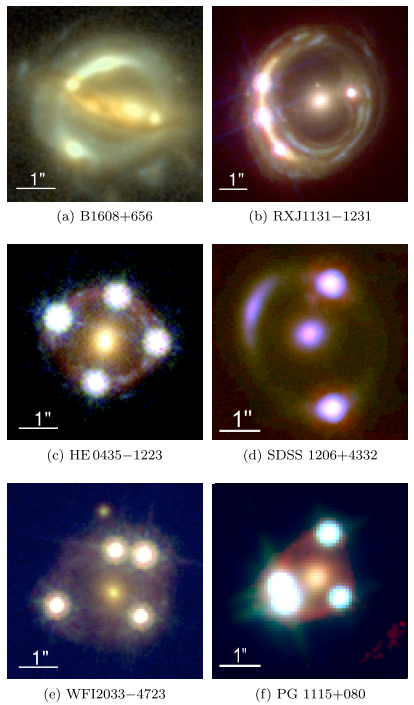
\includegraphics[width=0.25\textwidth]{holicow_lens}
                \caption{Mesure semi-directe: 
                $\boxed{100h = 73.3^{+1.7}_{-1.8}\,\,(2.4\%)}$ avec 
                        $z_\ell \sim 0.5$ et $z_s \lesssim 2$.
                \footnote{\citet{Wong2020}}}
        \end{figure}
\end{frame}

\subsection{Tension}
\begin{frame}{Tension}
        \begin{figure}[H]
                \centering
                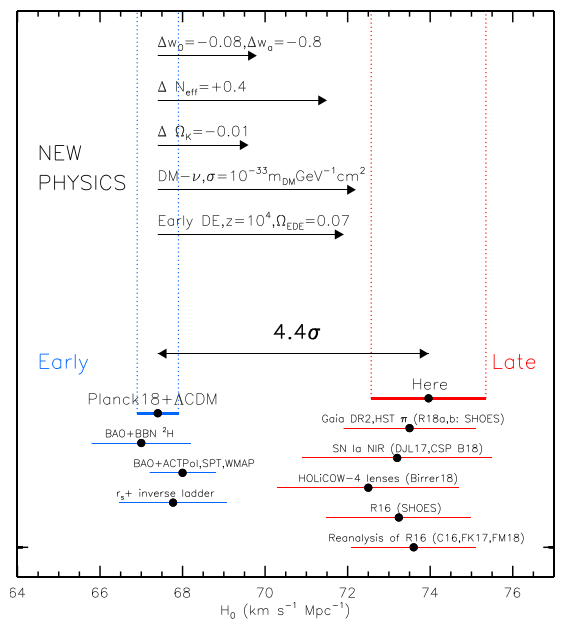
\includegraphics[width=0.4\textwidth]{H0_tension_Sh0es2019}
                \caption{
                        \footnote{\citet{Riess2019}}
                        Les mesures locales sont en conflit avec $H_0$ dérivée du CMB, 
                des oscillations acoustiques baryoniques (BAO) et de la nucléosynthèse 
        du Big Bang (BBN)}
        \end{figure}
         
\end{frame}

\section{Méthode}
\subsection{Équation du délai temporel}
\begin{frame}{Équation du délai temporel}
	\begin{equation}\label{eq:DelaiTemp} 
            \Delta t_{ij} = (1 + z_{\ell})\frac{D_\ell D_s}{D_{\ell s}c}
            \bigg[ \underbrace{\frac{(\theta_i - \beta)^2}{2} -
            \frac{(\theta_j - \beta)^2}{2}}_{\text{\citet{Refsdal1964}}} 
            -\underbrace{\psi(\theta_i) + \psi(\theta_j)}_{\text{\citet{Shapiro1964}}}
    \bigg]
	\end{equation}
La mesure de $H_0$ se fait via la \textit{distance caractéristique du délai temporel}
\begin{equation}\label{eq:Ddl} 
        D_{\Delta t} \equiv (1 + z_\ell)\frac{D_\ell D_s}{D_{\ell s}} \propto \frac{c}{H_0} 
\end{equation} 
On assume $\Lambda$CDM plat.
\end{frame}

\subsection{Théorie des lentilles gravitationnelles}
\begin{frame}{Théorie des lentilles gravitationnnelles}{Potentiel de Fermat}
Le potentiel a comme source la densité (baryonique) projeté sur le plan de la lentille. On doit donc résoudre une équation de Poisson:
\begin{equation}\label{eq:Poisson} 
        \laplacian_{\boldsymbol{\theta}} \psi = 2 \kappa(\boldsymbol{\theta}) 
\end{equation} 
       \begin{equation}\label{eq:potentiel} 
               \psi(\theta) = \frac{1}{\pi}\int_{\mathbb{R}^2} \kappa(\boldsymbol{\theta}')
               \ln(\boldsymbol{\theta} - \boldsymbol{\theta}') d^2\boldsymbol{\theta}'
       \end{equation}  
$\kappa$ est la \textit{convergence}, soit une mesure adimensionnelle de la densité de 
surface projeté sur le plan de la lentille 
\begin{equation}\label{eq:Kappa} 
        \kappa \equiv \frac{\Sigma}{\Sigma_{\text{cr}}},\hspace{1cm}
       \Sigma_{\text{cr}} \equiv \frac{c^2}{4 \pi G} 
       \frac{D_s}{D_\ell D_{\ell s}}
\end{equation} 
\end{frame}


\begin{frame}{Théorie des lentilles gravitationnelles}{Équation de la lentille}
\begin{minipage}{0.45\textwidth}
        \begin{figure}[H]
                \centering
                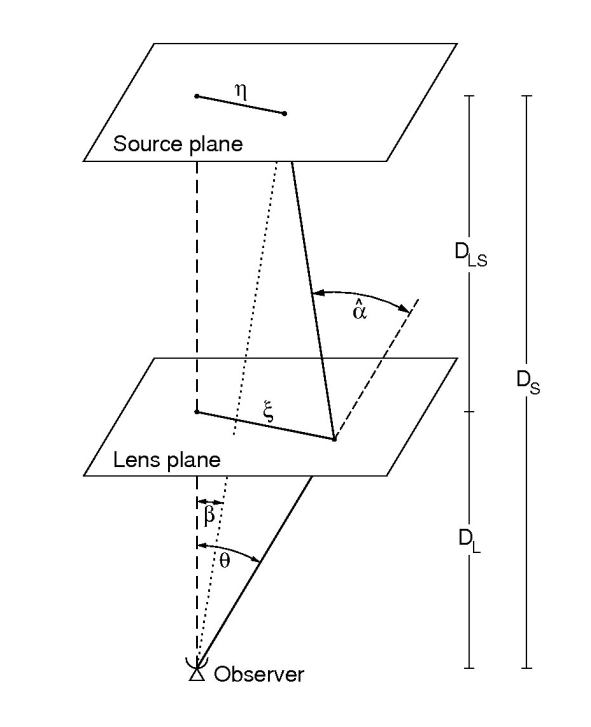
\includegraphics[width=0.8\textwidth]{lens_system_sketch}
                \caption{Sketch d'une lentille gravitationnelle \citet{Bartelmann2001}}
        \end{figure}
\end{minipage}
~
\begin{minipage}{0.5\textwidth}
L'image lentillée est obtenu via l'équationde la lentille:
\begin{equation}\label{eq:Lens Eq} 
        \boldsymbol{\beta} = \boldsymbol{\theta} - \boldsymbol{ \alpha}(\boldsymbol{ \theta} ) 
\end{equation} 
        Les angles de déflections sont obtenus en prenant le gradient du potentiel:
        \begin{equation}\label{eq:DeflectionAngles} 
                \boldsymbol{\alpha}(\boldsymbol{\theta}) 
                = \frac{1}{\pi}\int_{\mathbb{R}^2} \kappa(\boldsymbol{\theta}')
                \frac{\boldsymbol{\theta} -\boldsymbol{\theta}' }{
                |\boldsymbol{\theta} -\boldsymbol{\theta}' |}
                d^2\boldsymbol{\theta} 
        \end{equation} 
        
\end{minipage}
\end{frame}

\subsection{Modèle pour le potentiel de Fermat}

\section{RXJ1131-1231}
\begin{frame}
		
\end{frame}

\begin{frame}[allowframebreaks]{Références}
        \bibliography{bibliography.bib}
        
\end{frame}

\end{document}

